\documentclass[a4paper, 12pt]{extarticle}

% Поля
%--------------------------------------
\usepackage{geometry}
\geometry{a4paper,tmargin=2cm,bmargin=2cm,lmargin=3cm,rmargin=1cm}
%--------------------------------------


%Russian-specific packages
%--------------------------------------
\usepackage[T2A]{fontenc}
\usepackage[utf8]{inputenc} 
\usepackage[english, main=russian]{babel}
%--------------------------------------

\usepackage{textcomp}

% Красная строка
%--------------------------------------
\usepackage{indentfirst}               
%--------------------------------------             


%Graphics
%--------------------------------------
\usepackage{graphicx}
\graphicspath{ {./images/} }
\usepackage{wrapfig}
\usepackage{minted}
%--------------------------------------

% Полуторный интервал
%--------------------------------------
\linespread{1.3}                    
%--------------------------------------

%Выравнивание и переносы
%--------------------------------------
% Избавляемся от переполнений
\sloppy
% Запрещаем разрыв страницы после первой строки абзаца
\clubpenalty=10000
% Запрещаем разрыв страницы после последней строки абзаца
\widowpenalty=10000
%--------------------------------------

%Списки
\usepackage{enumitem}

%Подписи
\usepackage{caption} 

%Гиперссылки
\usepackage{hyperref}

\hypersetup {
	unicode=true
}

%Рисунки
%--------------------------------------
\DeclareCaptionLabelSeparator*{emdash}{~--- }
\captionsetup[figure]{labelsep=emdash,font=onehalfspacing,position=bottom}
%--------------------------------------

\usepackage{tempora}
\usepackage{amsmath}
\usepackage{color}
\usepackage{listings}
\lstset{
  belowcaptionskip=1\baselineskip,
  breaklines=true,
  frame=L,
  xleftmargin=\parindent,
  language=Python,
  showstringspaces=false,
  basicstyle=\footnotesize\ttfamily,
  keywordstyle=\bfseries\color{blue},
  commentstyle=\itshape\color{purple},
  identifierstyle=\color{black},
  stringstyle=\color{red},
}

%--------------------------------------
%			НАЧАЛО ДОКУМЕНТА
%--------------------------------------

\begin{document}

%--------------------------------------
%			ТИТУЛЬНЫЙ ЛИСТ
%--------------------------------------
\begin{titlepage}
\thispagestyle{empty}
\newpage


%Шапка титульного листа
%--------------------------------------
\vspace*{-30 pt}
\hspace{-65pt}
\begin{minipage}{0.3\textwidth}
\hspace*{-20pt}\centering

\includegraphics[width=60pt]{emblem}
\end{minipage}
\begin{minipage}{0.67\textwidth}\small \textbf{
\vspace*{-0.7ex}
\hspace*{-6pt}\centerline{Министерство науки и высшего образования Российской Федерации}
\vspace*{-0.7ex}
\centerline{Федеральное государственное бюджетное образовательное учреждение }
\vspace*{-0.7ex}
\centerline{высшего образования}
\vspace*{-0.7ex}
\centerline{<<Московский государственный технический университет}
\vspace*{-0.7ex}
\centerline{имени Н.Э. Баумана}
\vspace*{-0.7ex}
\centerline{(национальный исследовательский университет)>>}
\vspace*{-0.7ex}
\centerline{(МГТУ им. Н.Э. Баумана)}}
\end{minipage}
%--------------------------------------

\vspace{10pt}
\hspace{-35pt} \noindent \small ФАКУЛЬТЕТ\hspace{80pt} <<Информатика и системы управления>>

\vspace*{-16pt}
\hspace{47pt}\rule{0.83\textwidth}{0.4pt}

\vspace{0.5ex}
\hspace{-35pt} \noindent \small КАФЕДРА\hspace{50pt} <<Теоретическая информатика и компьютерные технологии>>

\vspace*{-16pt}
\hspace{30pt}\rule{0.866\textwidth}{0.4pt}
  
\vspace{6em}

\begin{center}
\Large {\bf Лабораторная работа №7} \\ 
\large {\bf по курсу <<Языки и методы программирования>>} \\ 
\large «Разработка простейшего класса на C++» \\
\large <<Вариант 22>>
\end{center}\normalsize

\vspace{15em}


\begin{flushright}
  {Студент группы ИУ9-21Б: Пенкин А. Д.\hspace*{15pt} \\
  \vspace{2ex}
  Преподаватель: Посевин Д. П.\hspace*{15pt}}
\end{flushright}

\bigskip

\vfill
 \vspace{7em}

\begin{center}
\textsl{Москва 2023}
\end{center}
\end{titlepage}
%--------------------------------------
%		КОНЕЦ ТИТУЛЬНОГО ЛИСТА
%--------------------------------------

\renewcommand{\ttdefault}{pcr}

\setlength{\tabcolsep}{3pt}
\newpage
\setcounter{page}{2}

\section{Цель}\label{Sect::task}
\par
Целью данной работы является изучение базовых объектно-ориентированных
возможностей языка C++. 
\section{Условие}
\par
Выполнение лабораторной работы заключается в составлении на языке C++
программы, состоящей из трёх файлов:
1. заголовочный файл MyString.h с объявлением класса;
2. файл MyString.cpp с определениями методов класса;
3. файл lab7.0.cpp, содержащий функцию main и, возможно, вспомогательные
функции для проверки работоспособности класса. 
\par
Последовательность символов ASCII с операциями:
1. получение количества символов;
2. получение ссылки на i-тый символ;
3. вставка нового символа в i-тую позицию
последовательности;
4. проверка, является ли последовательность
палиндромом. 
\section{Код решения}
1. lab7.0.cpp
\begin{minted}{c++}
#include <iostream>
#include "MyString.h"

int main()
{
	setlocale(LC_ALL, "Russian");
	char a[3] = { 'a', 'b', 'c' };
	MyString* axe = new MyString(a, 3);

	for (int i = 0; i < axe->len(); i++) {
		std::cout << axe->access(i) << " ";
	}

	std::cout << "\nСоздали строку из символов a b c\n";

	int count = 0;
	while (!axe->polyndrom() && count < 5) {
		axe->setChar(0, axe->access(0) + 1);
		for (int i = 0; i < axe->len(); i++) {
			std::cout << axe->access(i) << " ";
		}
		count++;
		std::cout << "\n";
	}

	std::cout << "Заменяли первый символ на следущий в \n";
	std::cout << "ASCII пока не получится полиндром\n\n";
	std::cout << "добавим элементов в строку:\n";
	axe->pushChar(0, 'a');
	axe->pushChar(1, 'b');
	for (int i = 0; i < axe->len(); i++) {
		std::cout << axe->access(i) << " ";
	}
	std::cout << "\n\nСоздадим второй класс и скопируем";
	std::cout << "\nданные из первого, выведем его:";


	MyString* diamond = new MyString();
	diamond->copy(axe);
	for (int i = 0; i < diamond->len(); i++) {
		std::cout << diamond->access(i) << " ";
	}
	std::cout << "\n";

	return 0;
}
\end{minted}
2. MyString.cpp
\begin{minted}{c++}
#include "MyString.h"


MyString::MyString() {
	str = new char[0];
	length = 0;
}

MyString::MyString(char *a, int n) {
	this->str = new char[n];
	this->length = n;
	for (int i = 0; i < n; i++) {
		this->str[i] = a[i];
	}
}

char* MyString::getStr() { return str; }

int MyString::len() { return length; }

char& MyString::operator[](int i) { return this->str[i]; }

char& MyString::access(int i) { return this->str[i]; }

void MyString::setChar(int i, char x) { str[i] = x; }

void MyString::pushChar(int i, char x) { 
	char* s = new char[length + 1];
	this->length++;
	for (int j = 0; j < length; j++) {
		if (j < i) { s[j] = str[j]; }
		if (j == i) { s[j] = x; }
		if (j > i) { s[j] = str[j - 1]; }
	}
	delete str;
	this->str = s;
}

void MyString::copy(MyString* s) {
	char* buf = new char[s->len()];
	this->length = s->len();
	for (int i = 0; i < length; i++) {
		buf[i] = s->access(i);
	}
	this->str = buf;
}

bool MyString::polyndrom() {
	bool res = true;
	for (int i = 0; 2 * i < length; i++) {
		if (str[i] != str[length - i - 1])
			res = false;
	}
	return res;
}

\end{minted}

3. MyString.h
\begin{minted}{c++}
#pragma once

class MyString
{
private:
	char* str;
	int length;
public:
	MyString(char *a, int n);
	MyString();
	char* getStr();
	int len();
	char& operator[](int i);
	char& access(int i);
	void setChar(int i, char x);
	void pushChar(int i, char x);
	bool polyndrom();
	~MyString();
	void copy(MyString* s);
};
\end{minted}

\section{Результаты работы программы}
\begin{figure}[H]
    \centering
    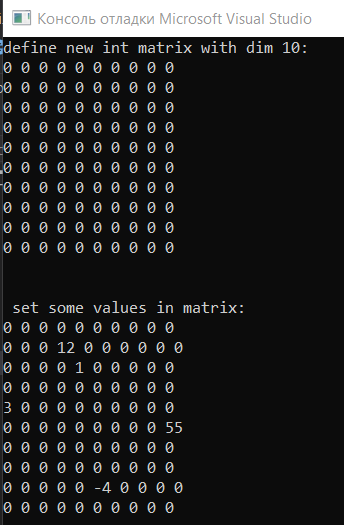
\includegraphics[width=400pt]{Test.png}
    \caption{создание строки и её вывод}
    \label{fig:my_label}
\end{figure}

\begin{figure}[H]
    \centering
    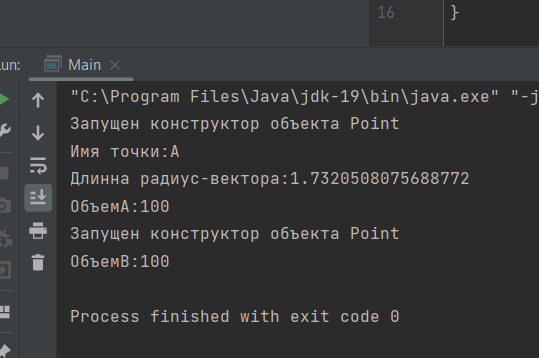
\includegraphics[width=400pt]{Test1.png}
    \caption{проверка методов polyndrom() и setChar()}
    \label{fig:my_label}
\end{figure}

\begin{figure}[H]
    \centering
    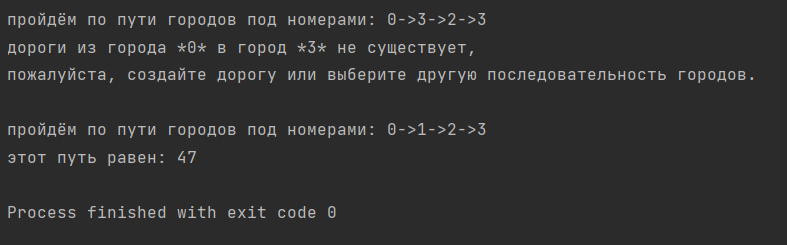
\includegraphics[width=400pt]{Test2.png}
    \caption{добавление элементов}
    \label{fig:my_label}
\end{figure}

\begin{figure}[H]
    \centering
    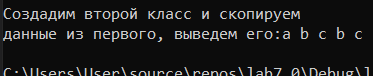
\includegraphics[width=400pt]{Test3.png}
    \caption{создание и копирование объекта класса}
    \label{fig:my_label}
\end{figure}


\end{document}